\documentclass{article}
\usepackage{graphicx} % Required for inserting images
\usepackage{hyperref} % Required for inserting links

\title{Rapport}
\author{Martin Rialhe-Badet}
\date{December 2023}

\begin{document}

\maketitle

\newpage

\subsection*{Introduction}

Ce rapport reprend les figures présentées lors de la réunion du 20 décembre 2023, accompagnées d'explications.

\section{Figures}

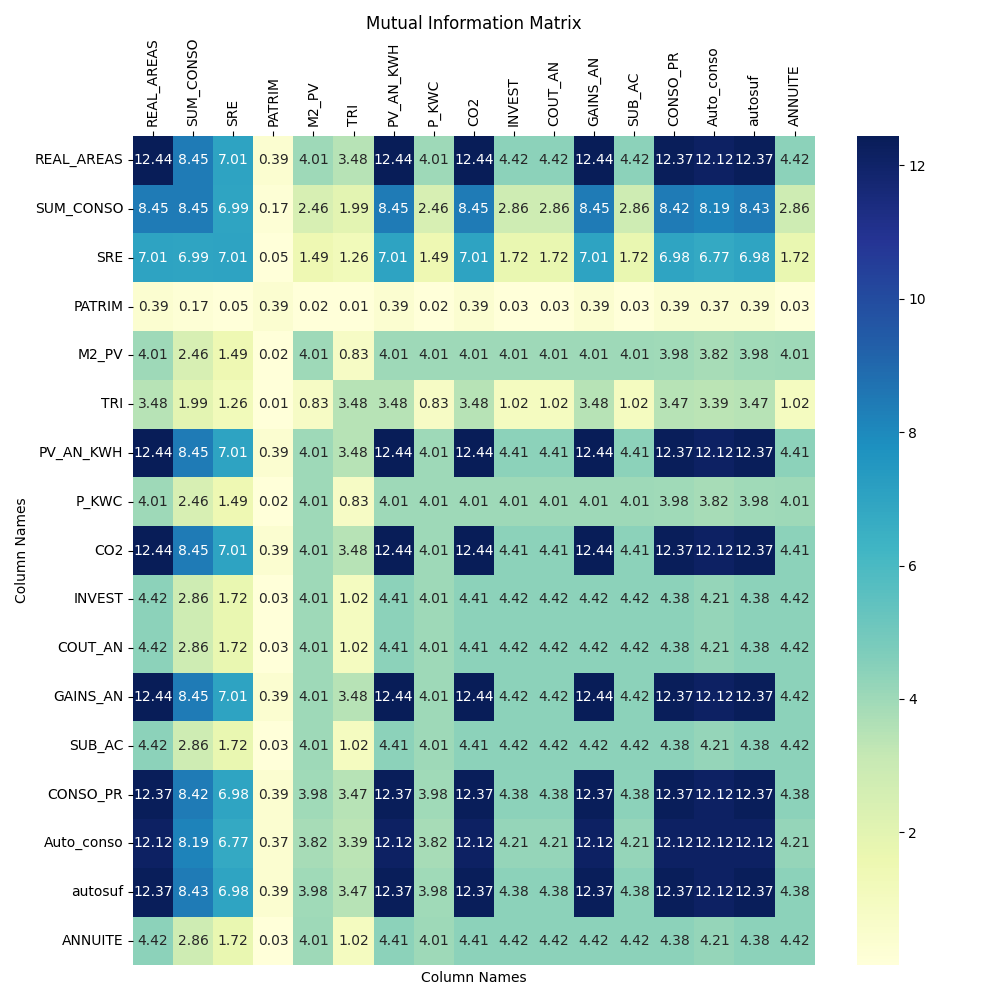
\includegraphics[width=\textwidth]{figures/mutual_information_matrix.png}

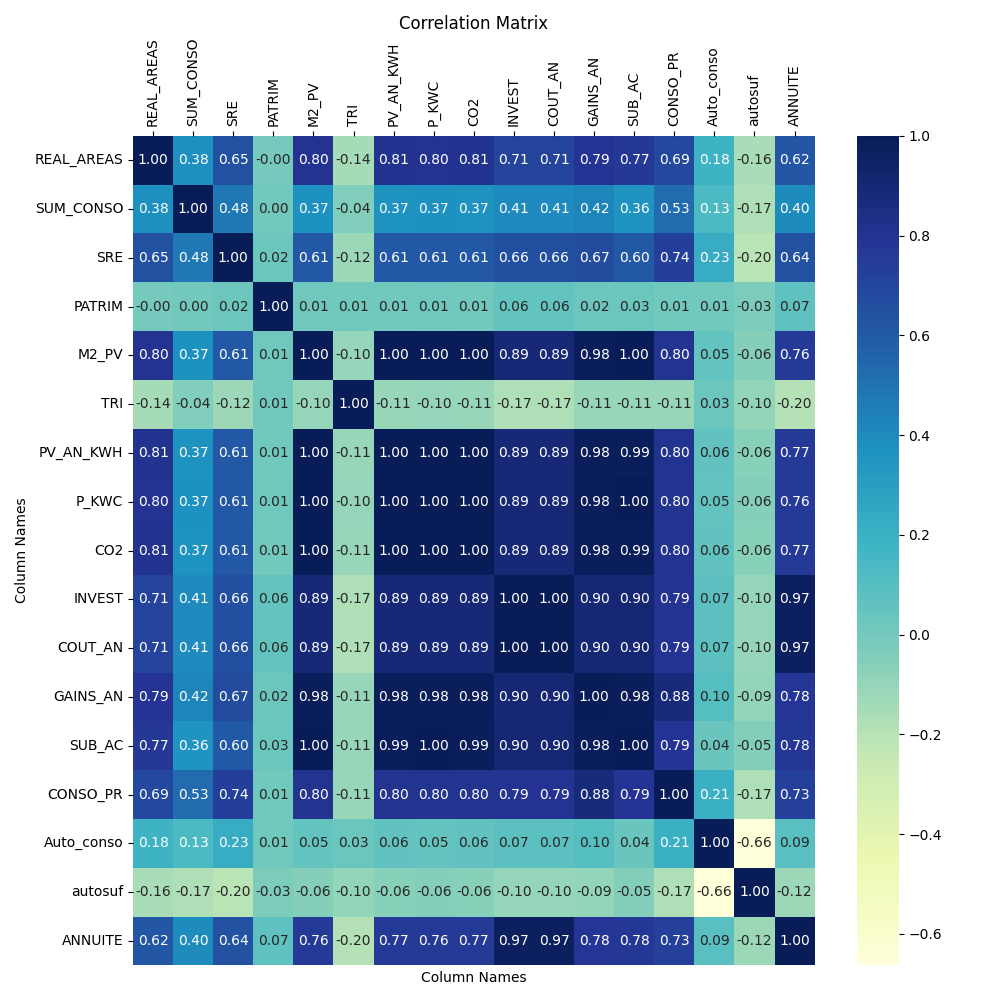
\includegraphics[width=\textwidth]{figures/correlation_matrix.png}

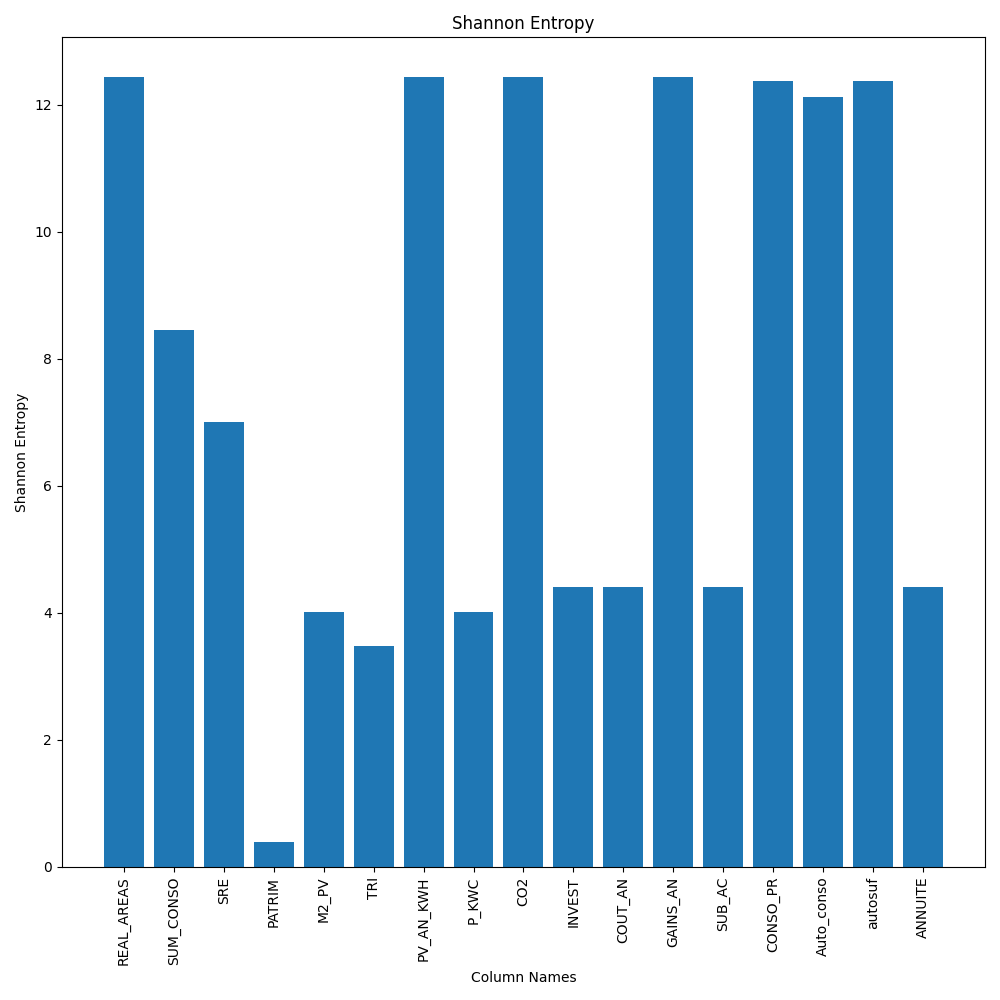
\includegraphics[width=\textwidth]{figures/shannon_entropy.png}

\section{Données}

Ces figures ont été obtenues à partir des données fournies par Martin Thébault (uniquement les colonnes à valeurs numériques).

Pour rappel, ces colonnes sont les suivantes :

\begin{itemize}
    \item \textbf{REAL\_AREAS} : surfaces exploitables totales du bâtiment (irradiation supérieure à un seuil de 800 ou 1000 kWh/m2/an) en m2 (issues du SITG) ;
    \item \textbf{SUM\_CONSO} : consommation totale du bâtiment en kWh ;
    \item \textbf{SRE} : surface de référence énergétique du bâtiment en m2 ;
    \item \textbf{PATRIM} : classification de la protection du bâtiment (0 : aucune, 1 : difficile d'installer des panneaux solaires, 2 : impossible d'installer des panneaux solaires) ;
    \item \textbf{M2\_PV} : surface de panneaux solaires photovoltaïques à installer pour maximiser le TRI en m2 ;
    \item \textbf{TRI} : temps de retour sur investissement en années ;
    \item \textbf{PV\_AN\_KWH} : production annuelle correspondant aux M2\_PV en kWh ;
    \item \textbf{PV\_KWC} : puissance installée correspondant aux M2\_PV en kW ;
    \item \textbf{CO2} : émissions de CO2 évitées en installant les M2\_PV en kg ;
    \item \textbf{INVEST} : investissement nécessaire pour installer les M2\_PV en EUR ;
    \item \textbf{COUT\_AN} : coût de maintenance annuel des M2\_PV en EUR (estimé à 1\% de l'investissement) ;
    \item \textbf{GAINS\_AN} : gains annuels en EUR ;
    \item \textbf{SUB\_AC} : subventions accordées par l'Etat en EUR ;
    \item \textbf{CONSO\_PROPRE} : consommation propre du bâtiment en kWh ;
    \item \textbf{Auto\_conso} : autoconsommation du bâtiment (rapport entre la consommation propre et la production) ;
    \item \textbf{autosuf} : autosuffisance du bâtiment (rapport entre la consommation propre et la consommation totale) ;
    \item \textbf{ANNUITE} : annuité du projet en EUR.
\end{itemize}

L'article est disponible \href{https://hal.science/hal-04234874/}{ici}.

\section{Interprétation}

\subsection{Matrice d'information mutuelle}

L'information mutuelle est une mesure de la dépendance entre deux variables aléatoires.
Les cases claires (presque nulles) indiquent des variables indépendantes, tandis que les cases plus foncées indiquent des variables fortement dépendantes.
On observe notamment une forte dépendance entre les variables des deux derniers tiers de la liste, qui ont été calculées à partir des variables précédentes.

\subsection{Matrice de corrélation}

La corrélation est une mesure de la dépendance linéaire entre deux variables aléatoires.
Les cases vertes (presque nulles) indiquent des variables non linéairement dépendantes, les cases foncées (proches de 1) indiquent des variables proportionnelles, et les cases claires (négatives) indiquent des variables inversement proportionnelles.
On retrouve ici Des dépendances importantes puisque les variables sont issues de calculs les unes à partir des autres.

\subsection{Entropie de Shannon}

L'entropie de Shannon est une mesure de la quantité d'information contenue dans une variable aléatoire.
Les variables qui ont une entropie faible sont celles qui ont peu de valeurs différentes.

\section{Code}

Le code qui a permis de générer ces figures, ainsi que les données utilisées, sont disponibles \href{https://github.com/MartinRB45534/Analyse-variables-pour-20231220}{ici}.

\end{document}
